% Created 2017-12-11 lun 15:00
% Intended LaTeX compiler: pdflatex
\documentclass[xcolor={usenames,svgnames,dvipsnames}]{beamer}
\usepackage[utf8]{inputenc}
\usepackage[T1]{fontenc}
\usepackage{graphicx}
\usepackage{grffile}
\usepackage{longtable}
\usepackage{wrapfig}
\usepackage{rotating}
\usepackage[normalem]{ulem}
\usepackage{amsmath}
\usepackage{textcomp}
\usepackage{amssymb}
\usepackage{capt-of}
\usepackage{hyperref}
\usepackage{color}
\usepackage{listings}
\usepackage{mathpazo}
\usepackage{gensymb}
\usepackage{amsmath}
\bibliographystyle{plain}
\AtBeginSubsection[]{\begin{frame}[plain]\tableofcontents[currentsubsection,sectionstyle=show/shaded,subsectionstyle=show/shaded/hide]\end{frame}}
\AtBeginSection[]{\begin{frame}[plain]\tableofcontents[currentsection,hideallsubsections]\end{frame}}
\usepackage[emulate=units]{siunitx}
\sisetup{fraction=nice, decimalsymbol=comma, retain-unity-mantissa = false}
\newunit{\wattpeak}{Wp}
\newunit{\watthour}{Wh}
\newunit{\amperehour}{Ah}
\hypersetup{colorlinks=true, linkcolor=Blue, urlcolor=Blue}
\renewcommand{\thefootnote}{\fnsymbol{footnote}}
\setbeamercolor{alerted text}{fg=blue!50!black} \setbeamerfont{alerted text}{series=\bfseries}
\usetheme[hideothersubsections]{Goettingen}
\usecolortheme{rose}
\usefonttheme{serif}
\author{Oscar Perpiñán Lamigueiro \\ \url{http://oscarperpinan.github.io}}
\date{}
\title{Energía Solar Fotovoltaica}
\subtitle{Aplicaciones y Contexto Mundial}
\hypersetup{
 pdfauthor={Oscar Perpiñán Lamigueiro \\ \url{http://oscarperpinan.github.io}},
 pdftitle={Energía Solar Fotovoltaica},
 pdfkeywords={},
 pdfsubject={},
 pdfcreator={Emacs 25.2.2 (Org mode 9.1.2)}, 
 pdflang={Spanish}}
\begin{document}

\maketitle

\section{Aplicaciones de la Energía Solar Fotovoltaica}
\label{sec:org6c56168}

\subsection{Clasificación}
\label{sec:org449f094}

\begin{frame}[label={sec:orgf003049}]{Definición}
\begin{itemize}
\item Un sistema fotovoltaico es el conjunto de equipos eléctricos y
electrónicos que producen energía eléctrica a partir de la radiación
solar.

\item El principal componente de este sistema es el módulo fotovoltaico, a
su vez compuesto por células capaces de transformar la energía
luminosa incidente en energía eléctrica de corriente continua.

\item El resto de equipos incluidos en un sistema fotovoltaico depende en
gran medida de la aplicación a la que está destinado.

\item Tipos
\begin{itemize}
\item Conectados a red (\emph{grid connected}),

\item autónomos (\emph{off-grid})

\item y de bombeo.
\end{itemize}
\end{itemize}
\end{frame}

\begin{frame}[label={sec:orgd9aac36}]{}
\begin{center}
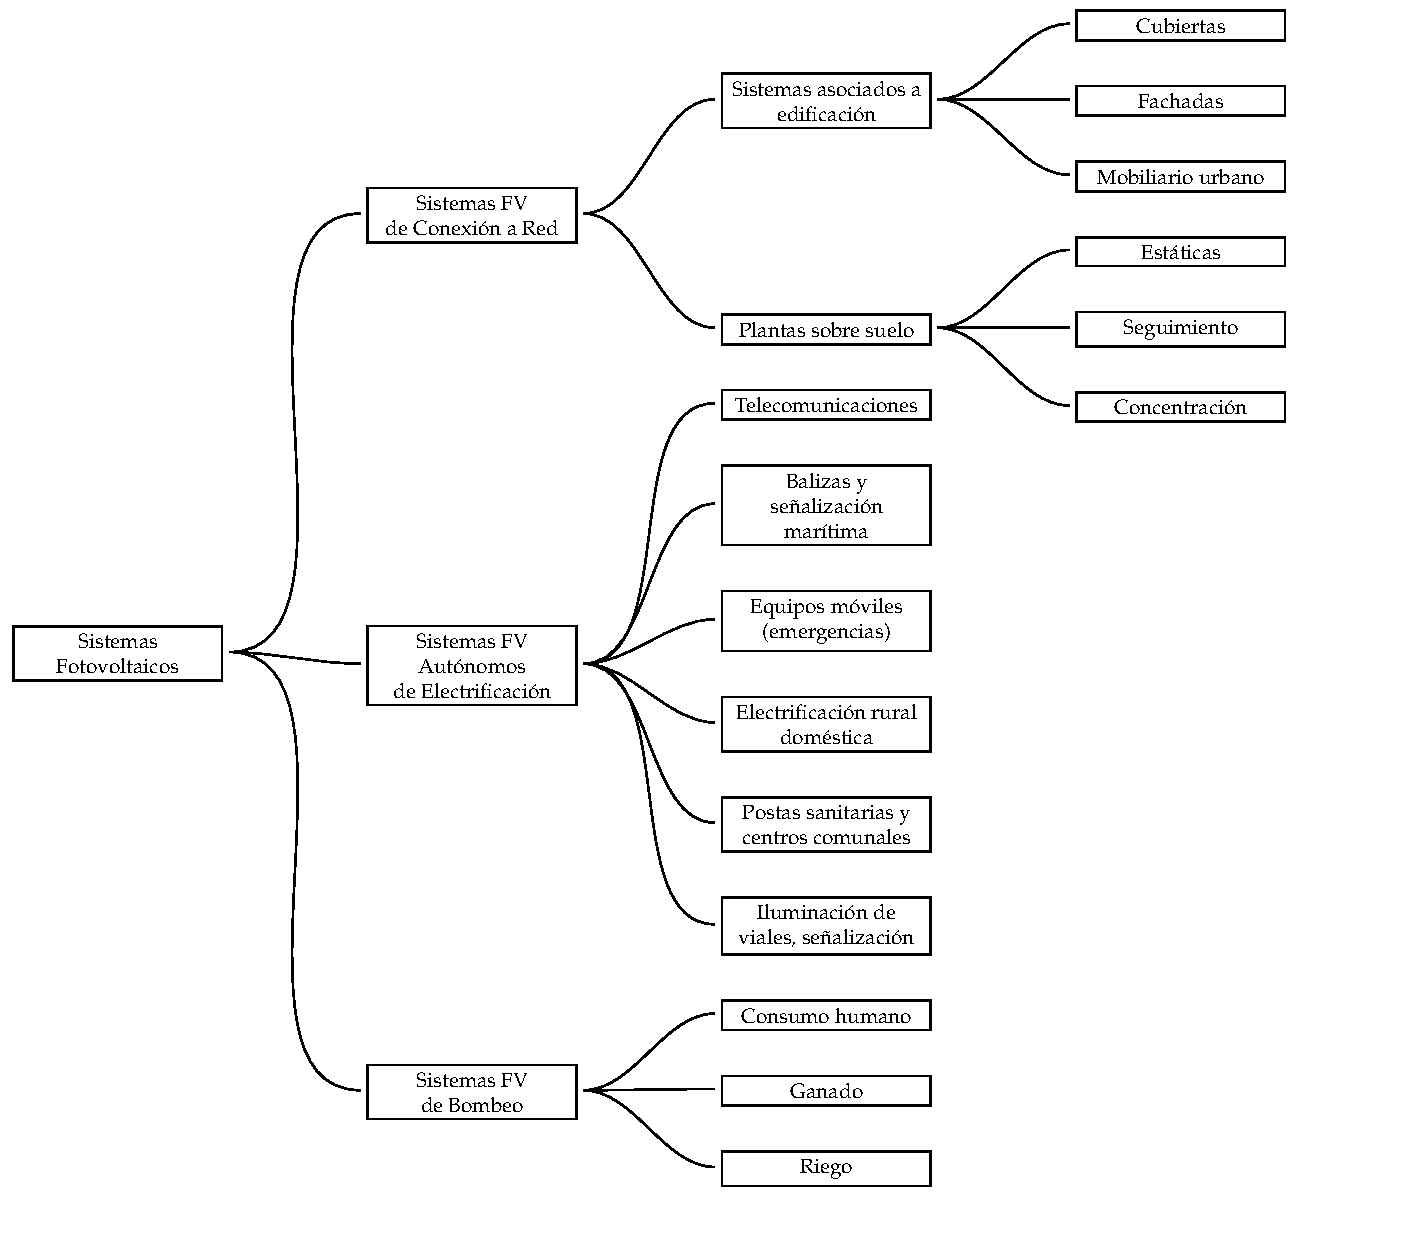
\includegraphics[width=.9\linewidth]{../figs/ClasificacionSistemas.pdf}
\end{center}
\end{frame}

\subsection{SFCR}
\label{sec:org60f0cab}

\begin{frame}[label={sec:org3721afa}]{Definición}
\begin{itemize}
\item Los sistemas conectados a red producen energía eléctrica para ser
inyectada íntegramente en la red convencional.

\item Dado que no deben satisfacer ninguna demanda de consumo de forma
directa ni garantizar el mismo, no necesitan incorporar equipos de
acumulación de energía.

\item Para permitir el correcto acoplamiento con la red eléctrica estos
sistemas incorporan un equipo inversor que adecúa la potencia
producida por el generador fotovoltaico a las condiciones de la red
convencional.
\end{itemize}
\end{frame}

\begin{frame}[label={sec:org8deed78}]{Tipos de SFCR}
\begin{itemize}
\item Estos sistemas pueden a su vez ser divididos en sistemas instalados
sobre suelo y sistemas en edificación.

\item Los sistemas sobre suelo, concebidos exclusivamente para producir
energía y obtener el rendimiento económico asociado, suelen superar
los \(\SI{100}{\kilo\watt}\) de potencia.

\item Los sistemas en edificación abarcan funciones adicionales a la
producción de energía, tales como sustitución de componentes
arquitectónicos, efecto estético, sombreado de acristalamientos,
etc.

\item En general, son sistemas más pequeños que los instalados sobre
suelo, normalmente de potencias inferiores a los
\(\SI{100}{\kilo\watt}\).
\end{itemize}
\end{frame}

\begin{frame}[label={sec:orgb4f6646}]{Estática sobre suelo}
\begin{center}
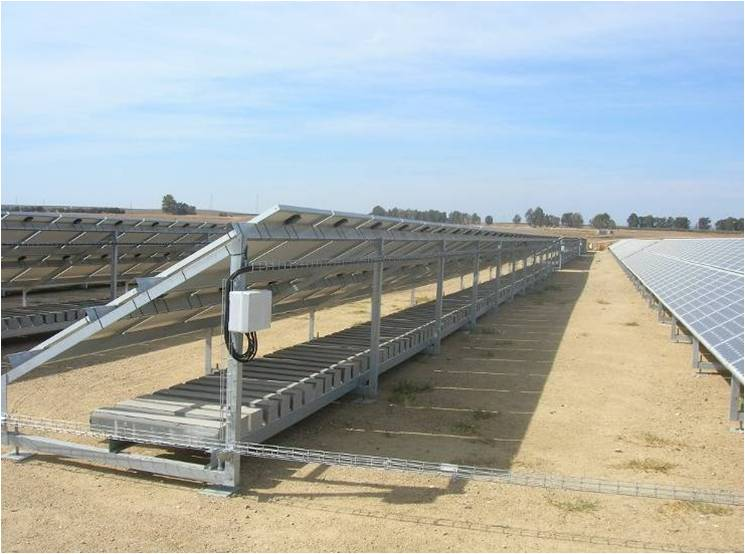
\includegraphics[width=.9\linewidth]{../figs/EstructuraEstaticaSuelo.jpg}
\end{center}
\end{frame}

\begin{frame}[label={sec:orgaec891f}]{Integración en edificios}
\begin{center}
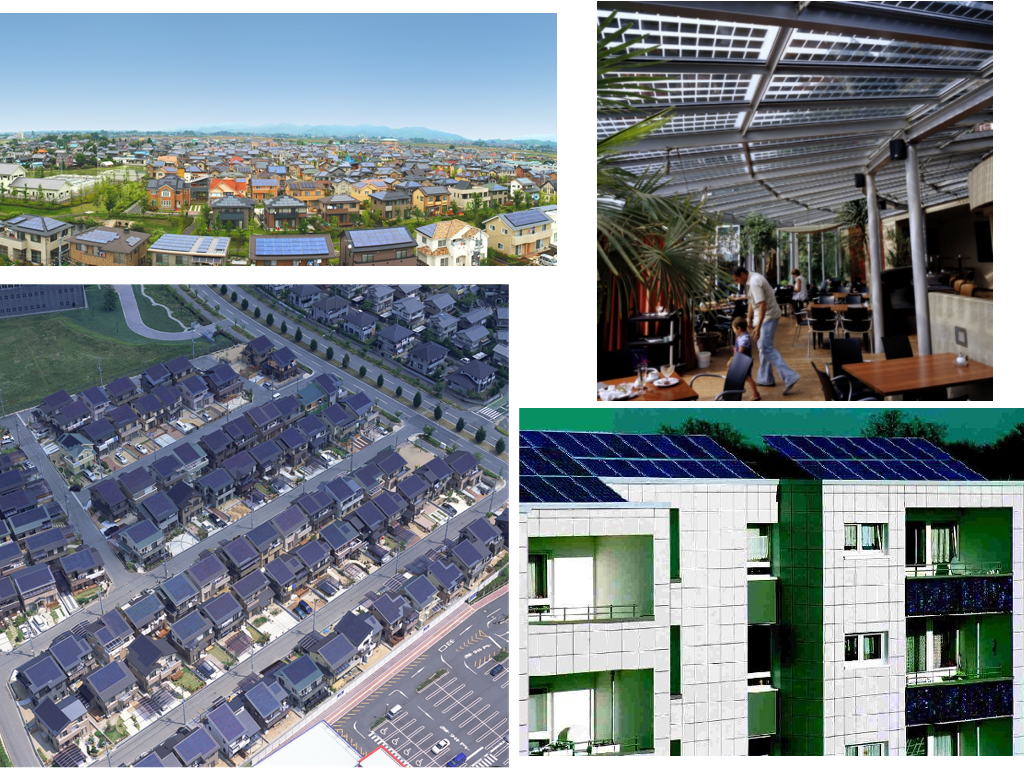
\includegraphics[width=.9\linewidth]{../figs/PVUrban.png}
\end{center}
\end{frame}

\subsection{Sistemas Autónomos}
\label{sec:org1120743}
\begin{frame}[label={sec:orge6f0fe4}]{Definición}
\begin{itemize}
\item Los sistemas autónomos abarcan una variedad muy amplia de
aplicaciones. Su denominador común es la necesidad de satisfacer una
demanda energética determinada.

\item Por esta razón, prácticamente todos los sistemas autónomos
incorporan un equipo de acumulación de energía.

\item Estos sistemas pueden ser clasificados en tres grupos por razón de
su aplicación asociada: profesionales, electrificación rural y
pequeño consumo.
\end{itemize}
\end{frame}

\begin{frame}[label={sec:org1b96b91}]{Aplicaciones profesionales}
\begin{itemize}
\item Las aplicaciones profesionales son variadas y abarcan campos tales
como los radioenlaces, la protección catódica de gasoductos,
hoteles, señales de tráfico y navegación aérea, refrigeración de
vacunas, equipos remotos de adquisición y transmisión de datos, e
incluso alimentación equipos espaciales como satélites.

\item Todas estas aplicaciones se caracterizan por requerir una fiabilidad
muy elevada.

\item Dado que el corte de suministro en estas aplicaciones tiene
consecuencias de elevado coste, suele optarse por incorporar un
generador fotovoltaico y un acumulador electroquímico de tamaño
superior al estrictamente necesario y así reducir al mínimo la
probabilidad de fallo.

\item En algunos casos se opta por incorporar un grupo electrógeno, ya sea
para reducir el tamaño del acumulador o para funcionar como equipo
de socorro.
\end{itemize}
\end{frame}

\begin{frame}[label={sec:org70190fb}]{}
\begin{center}
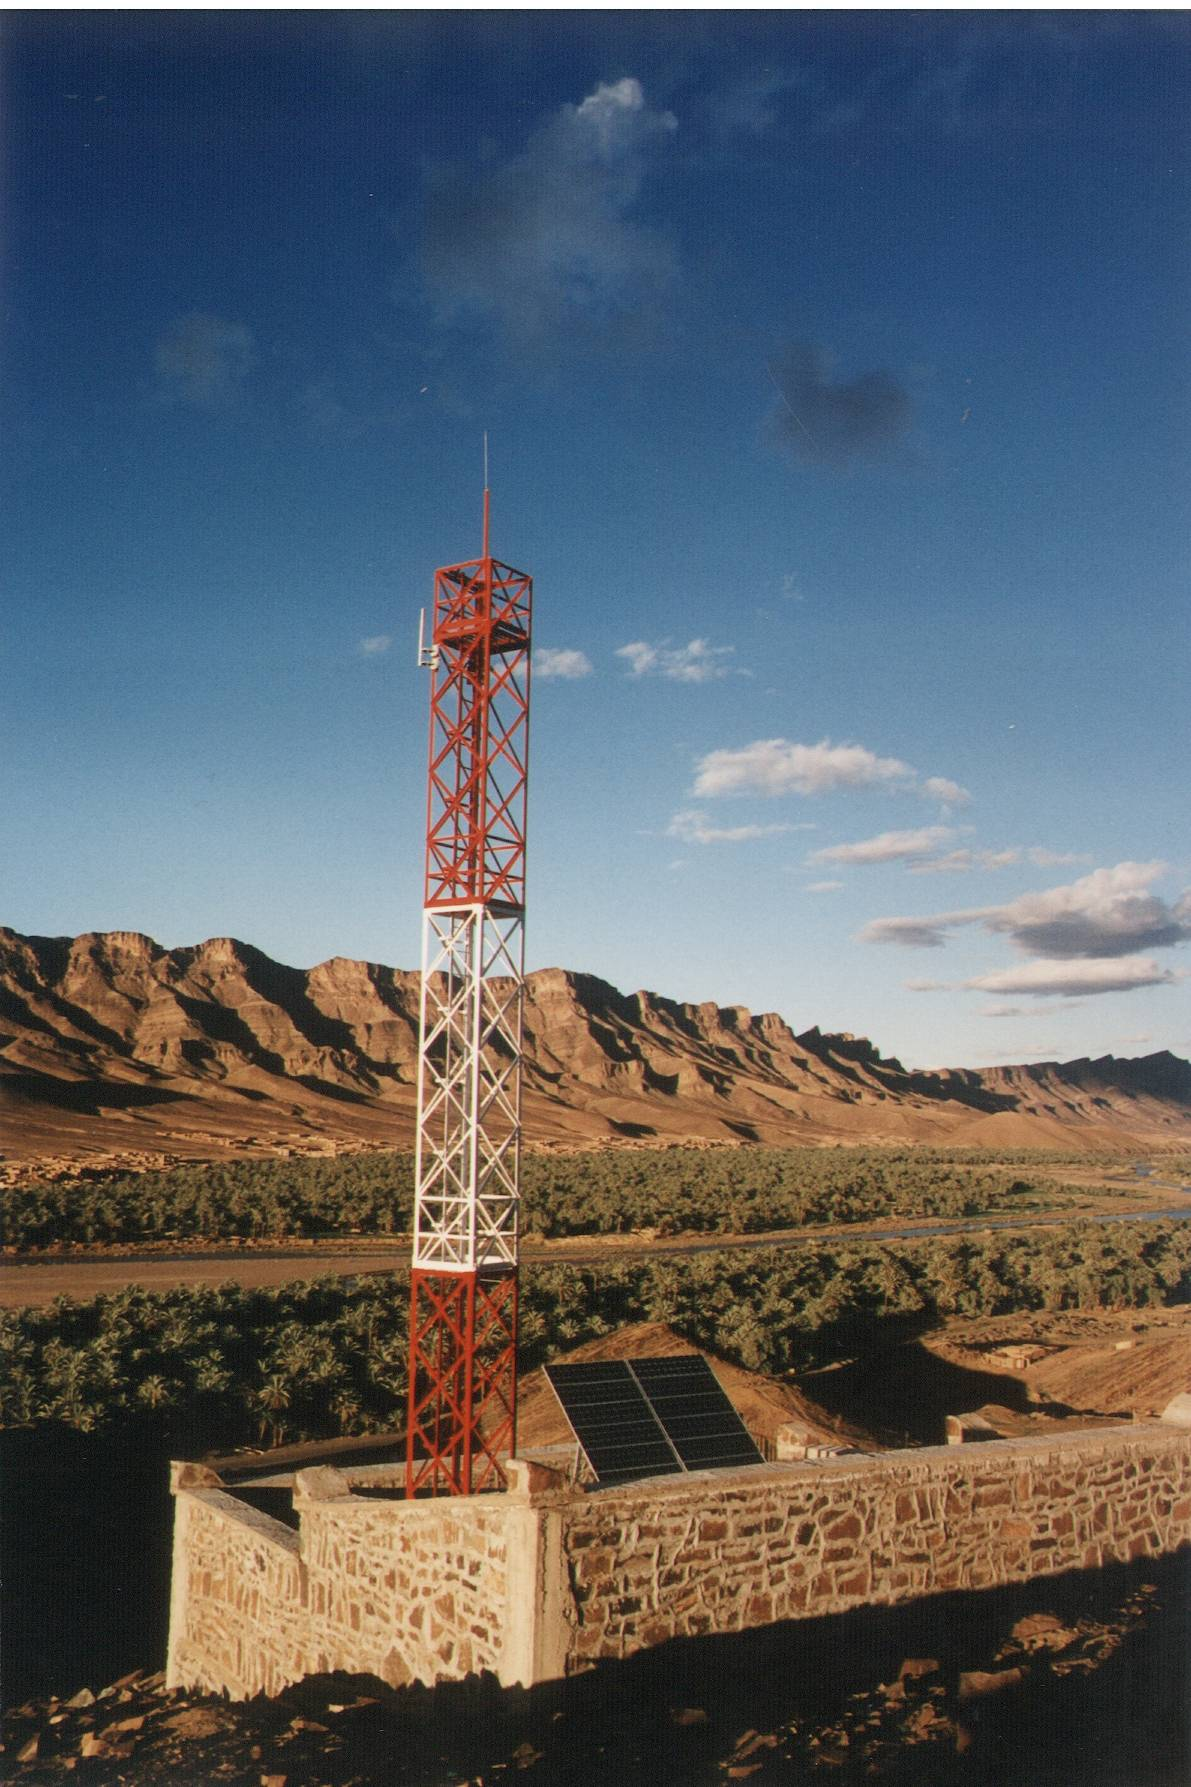
\includegraphics[height=0.95\textheight]{../figs/TelefoniaRural.jpg}
\end{center}
\end{frame}

\begin{frame}[label={sec:org9a746c9}]{Sistemas de Electrificación Rural}
\begin{itemize}
\item Los sistemas de electrificación rural suministran energía eléctrica
a poblaciones rurales alejadas de redes eléctricas convencionales.

\item Son sistemas frecuentemente englobados en programas de cooperación
al desarrollo, financiados por ONG's u organismos como el Banco
Mundial o la Unión Europea.

\item Dentro de los sistemas de electrificación rural predominan los
sistemas domésticos (\emph{solar home systems, SHS}), las centrales
híbridas y los sistemas de bombeo.

\item Tanto los sistemas domésticos como las centrales híbridas
proporcionan energía para alimentar equipos de iluminación, radio,
televisión y pequeñas herramientas eléctricas.
\end{itemize}
\end{frame}

\begin{frame}[label={sec:org18a997c}]{SHS}
\begin{itemize}
\item Los sistemas domésticos habitualmente con potencias de
\(\SI{100}{\watt}\) o \(\SI{200}{\watt}\), están asociados a una
vivienda familiar y en algunos casos a centros comunales o centros
de salud.
\end{itemize}

\begin{center}
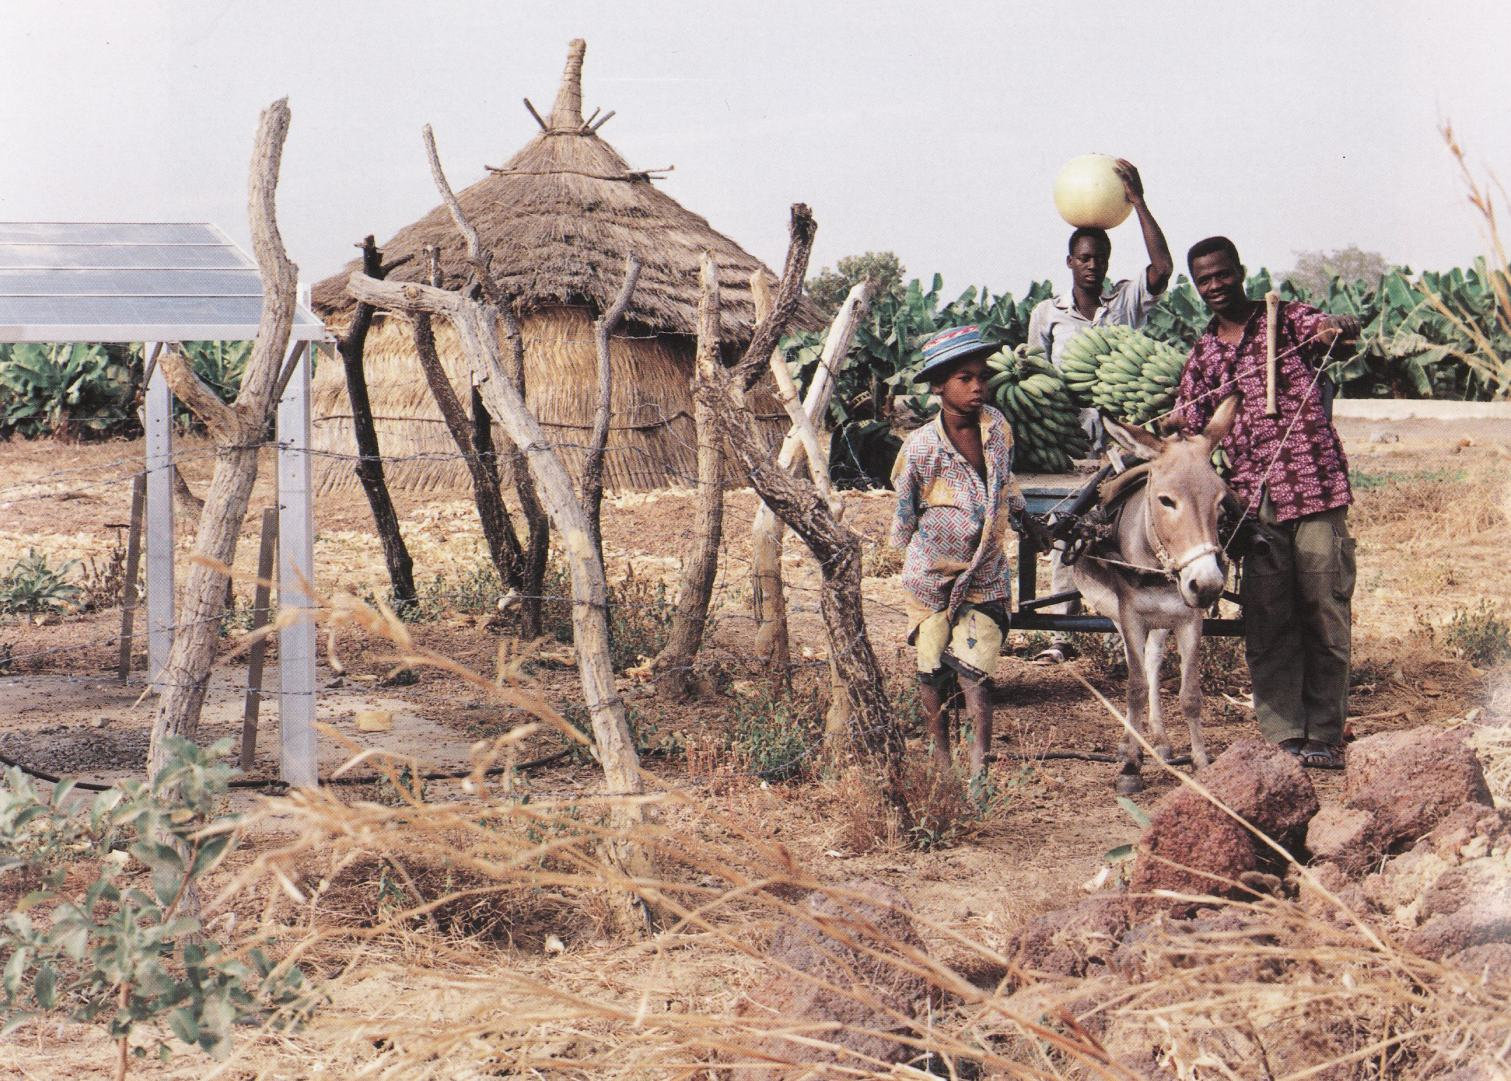
\includegraphics[width=.9\linewidth]{../figs/er.jpg}
\end{center}
\end{frame}


\begin{frame}[label={sec:org514394f}]{Híbridos}
\begin{itemize}
\item Las centrales híbridas, compuestas por un generador fotovoltaico, un
acumulador electroquímico y un grupo electrógeno o turbina eólica,
proveen una red eléctrica para un poblado rural.

\item El tamaño de estas centrales depende del tamaño de la población
asociada, con potencias que van desde los \(\SI{10}{\kilo\watt}\)
hasta los \(\SI{100}{\kilo\watt}\).
\end{itemize}
\end{frame}

\begin{frame}[label={sec:org0ab7c2a}]{Aplicaciones pequeño consumo}
Dentro de las aplicaciones de pequeño consumo se emplean pequeños
módulos fotovoltaicos, frecuentemente de silicio amorfo, alimentando
equipos electrónicos como calculadoras o relojes, cargadores de
móviles, pequeñas herramientas eléctricas, balizas domésticas, etc.
\end{frame}


\subsection{Sistemas de Bombeo}
\label{sec:org94278b8}
\begin{frame}[label={sec:org36dd43d}]{Definición}
\begin{itemize}
\item Los sistemas de bombeo emplean la energía eléctrica que produce el
generador fotovoltaico para accionar una motobomba que eleva y
transporta agua desde un acuífero hasta un depósito o una red de
distribución.

\item Para reducir costes y aumentar la fiabilidad, en estos sistemas es
frecuente acumular la energía en forma de energía potencial del agua
almacenada en el depósito elevado.

\item Las aplicaciones de los sistemas de bombeo incluyen el suministro de
agua para consumo humano o animal, el riego de plantaciones
individuales o comunitarias y la desalinización del agua extraída
con sistemas de ósmosis inversa.
\end{itemize}
\end{frame}
\begin{frame}[label={sec:org0c45b44}]{}
\begin{center}
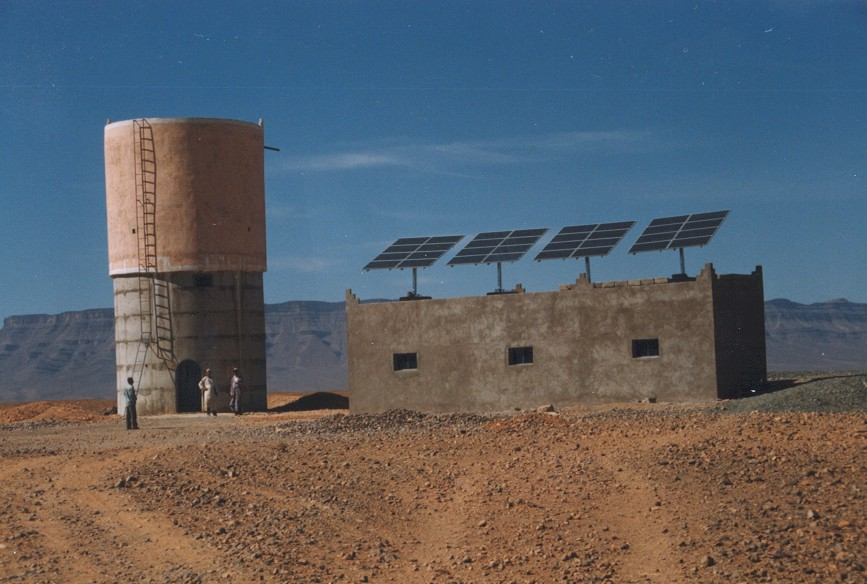
\includegraphics[width=.9\linewidth]{../figs/Bombeo.jpg}
\end{center}
\end{frame}

\section{Contexto Mundial}
\label{sec:orge0820db}

\subsection{Mercado Fotovoltaico}
\label{sec:orgd17d7fb}

\begin{frame}[label={sec:org353bb6f}]{Potencia Instalada}
Según el informe preliminar del mercado fotovoltaico publicado por la
Agencia Internacional de la Energía (IEA-PVPS) en 2014 había una
potencia fotovoltaica acumulada de \SI{177}{\giga\watt} a nivel
mundial.
\end{frame}

\begin{frame}[label={sec:orgce67e0a}]{Potencia por Países}
Hay 20 países que han superado la cifra de \SI{1}{\giga\watt} de
potencia instalada, destacando Alemania con \SI{38.2}{\giga\watt},
China con \SI{28.1}{\giga\watt}, Japón con \SI{23.3}{\giga\watt},
Italia con \SI{18.5}{\giga\watt}, Estados Unidos
\SI{18.3}{\giga\watt}, Francia con \SI{5.7}{\giga\watt}, España con
\SI{5.4}{\giga\watt}, y Reino Unido con \SI{5.1}{\giga\watt}.
\end{frame}

\begin{frame}[label={sec:org8426cbc}]{}
\begin{center}
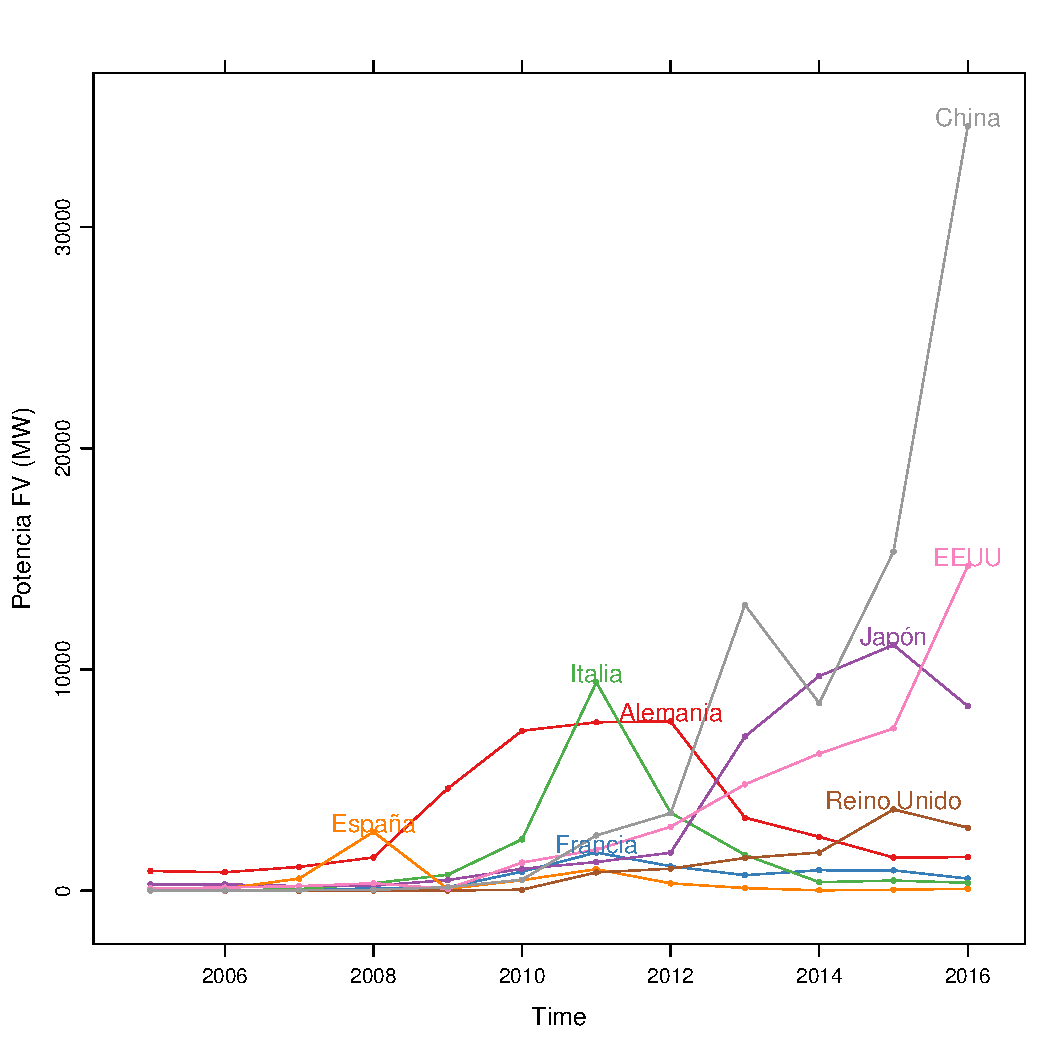
\includegraphics[width=.9\linewidth]{../figs/PVWorld.pdf}
\end{center}
\end{frame}


\begin{frame}[label={sec:org2891ce1}]{Contribución energética}
Este campo fotovoltaico aporta el 1\% de la energía eléctrica mundial,
destacando los casos particulares de Italia con el 7.9\% de su
electricidad nacional, Grecia con el 7.6\%, y Alemania con el 7\%.
\end{frame}

\subsection{Paridad de Red}
\label{sec:org52b267e}

\begin{frame}[label={sec:orgeb78aee}]{Paridad de Red}
\begin{itemize}
\item La situación actual es el resultado de un crecimiento sostenido
liderado por Alemania, China, Japón, y Estados Unidos, y la
contribución más inestable de otros países como España, Italia y
Reino Unido.

\item Este crecimiento está fuertemente relacionado con el ritmo de
reducción del precio del módulo, siendo causa y consecuencia del
mismo.

\item En estas circunstancias, los sistemas fotovoltaicos han alcanzado ya
la paridad de red en muchas partes del mundo.
\end{itemize}
\end{frame}


\begin{frame}[label={sec:org5b3a6f5}]{}
\begin{center}
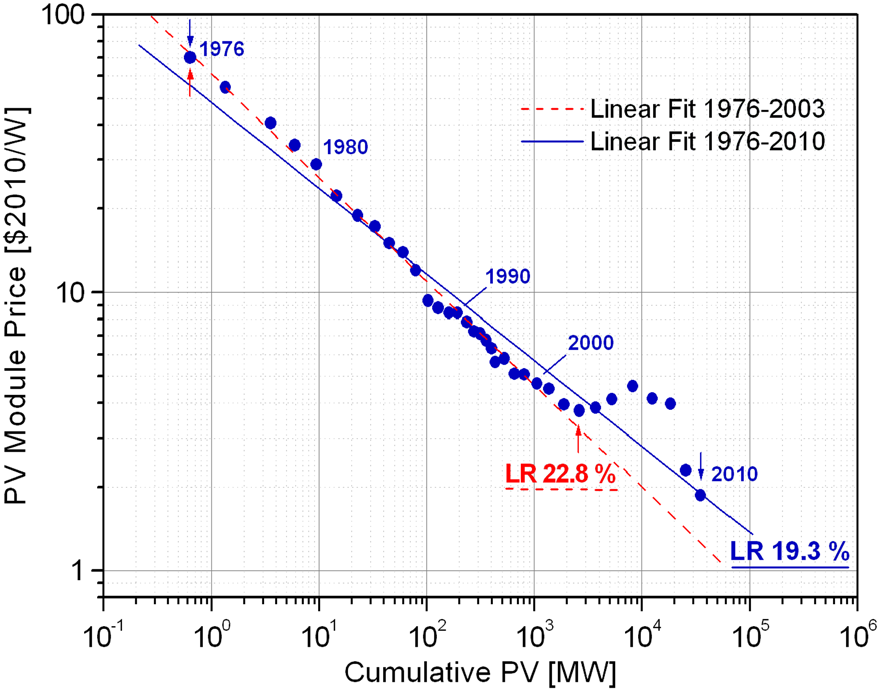
\includegraphics[width=.9\linewidth]{../figs/CurvaAprendizajeFV_BreyerPiP.png}
\end{center}
\end{frame}

\begin{frame}[label={sec:orga15f6cb}]{Paridad en 2010}
\begin{center}
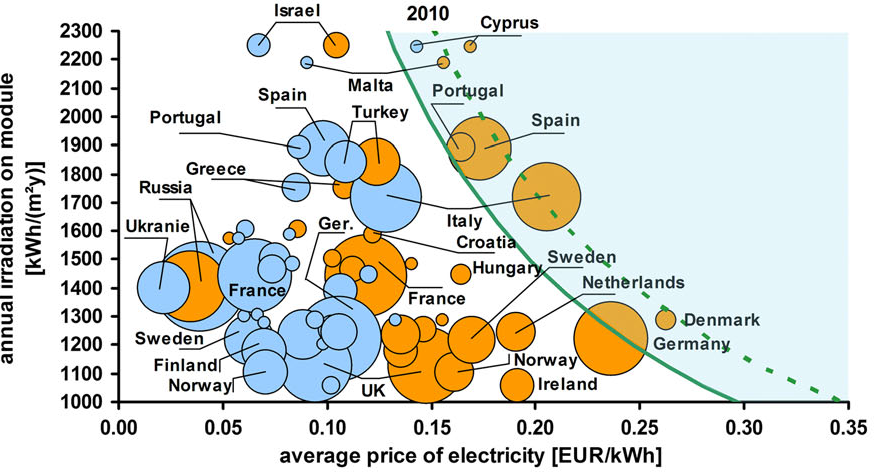
\includegraphics[width=.9\linewidth]{../figs/GridParity2010.png}
\end{center}
\end{frame}

\begin{frame}[label={sec:org6a4d931}]{Paridad en 2013}
\begin{center}
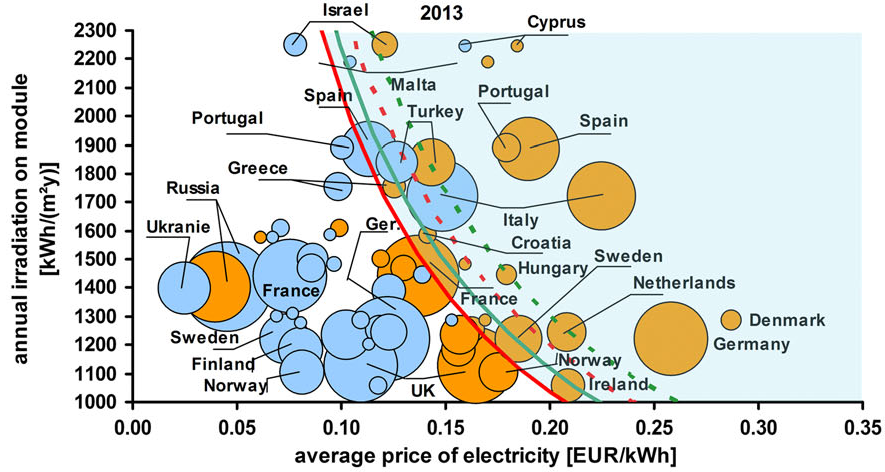
\includegraphics[width=.9\linewidth]{../figs/GridParity2013.png}
\end{center}
\end{frame}

\subsection{Segmentos de mercado}
\label{sec:org4f6e2f0}

\begin{frame}[label={sec:orgbd54e7c}]{Segmentos de Mercado}
\begin{itemize}
\item La European Photovoltaics Industry Association diferencia entre:
\begin{itemize}
\item sistemas sobre terreno,
\item sistemas en entorno industrial,
\item comercial,
\item y residencial.
\end{itemize}
\item Es destacable que el mercado fotovoltaico español se ha basado en
sistemas sobre terreno (plantas fotovoltaicas), mientras que el
mercado alemán ha diversificado las opciones dando mayor
preponderancia a sistemas comerciales y residenciales.
\end{itemize}
\end{frame}

\begin{frame}[label={sec:org65620aa}]{}
\begin{center}
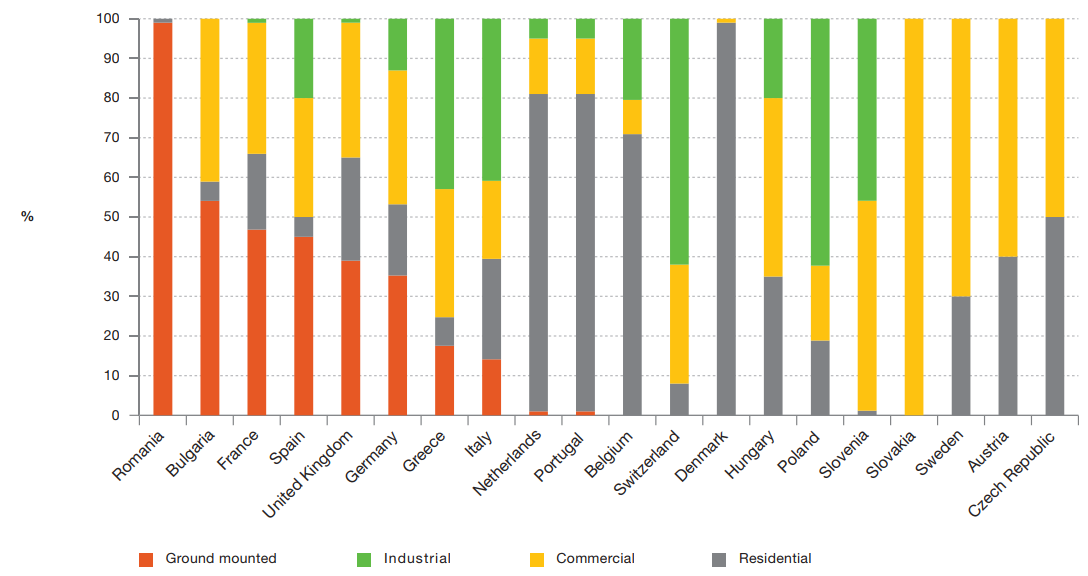
\includegraphics[width=.9\linewidth]{../figs/SegmentacionFVEuropa_EPIA.png}
\end{center}
\end{frame}

\begin{frame}[label={sec:orgaf36cae}]{Conexión a Red}
\begin{itemize}
\item Esta diferencia entre mercados puede observarse desde la óptica del
tamaño medio de las instalaciones y el tipo de conexión.
\item En España el tamaño medio de los sistemas fotovoltaicos instalados
es de \SI{107}{\kilo\watt}, con el 64\% de los sistemas conectados a
redes de Alta o Media Tensión, y el 36\% en redes de Baja Tensión.
\item En Alemania el tamaño medio de sistema es un orden de magnitud
menor, \SI{17}{\kilo\watt}, con el 38\% de los sistemas conectados en
redes de AT/MT, y el 62\% en BT.
\item Finalmente, en Japón el tamaño medio de los sistemas es aún menor,
sin superar los \SI{5}{\kilo\watt}, estando conectados en redes de
BT el 80\% del total.
\end{itemize}
\end{frame}
\end{document}